\documentclass[11pt,twoside,letterpaper]{book}	
%Archivo del preámbulo
\usepackage[utf8]{inputenc} %Ajustando codificacion de los caracteres 
\usepackage[spanish]{babel} %Para configurar le lenguaje
\usepackage{amsmath}
\usepackage{amsfonts}
\usepackage{amssymb}
\usepackage{makeidx} %Para crear índice alfabético
\usepackage{titlesec}
\titleformat{\chapter}[display]
{\normalfont\huge\bfseries}{}{0pt}{\Huge}
\makeindex
\usepackage{lipsum} %Para generar parrafos de ejemplo.
\usepackage{enumitem} %Para ajustar el estilo de los items enumerados.
\setlist[enumerate,1]{label=\arabic*.}
\usepackage{ragged2e} %Para justificar
\usepackage[top=2cm,bottom=2cm,inner=3cm,outer=2cm]{geometry} %Para modificar los margenes del documento.
%Seccion para teoremas y definiciones
\usepackage{amsthm}
\theoremstyle{plain}%definition,remark
\newtheorem{theorem}{Teorema}
\newtheorem{Def}{Definición}[section]
\newtheorem{Prop}[Def]{Proposición}
%-------------------------------------
%\usepackage{enumitem} %Para hacer ajustes a las listas
\usepackage{graphicx} %Paquete para insertar imagenes
\graphicspath{{./Imagenes/}}
\usepackage{float}% para ajustar la posición de un grafico o una tabla
%-------------------------------------
%Para referencias internas y externas
\usepackage{hyperref}
\hypersetup{
    colorlinks=true,
    linkcolor=blue,
    }
%Seccion para tablas
\usepackage{array}
\usepackage{multirow}
\usepackage{booktabs}%Para lineas especiales
\usepackage[table]{xcolor}%Para utilizar color
\usepackage{colortbl}%Para colo en tablas del entorno tabular
\usepackage{setspace}%Controlar espacio entre filas
\definecolor{color1}{RGB}{239,184,16}%Definiendo un color en el formato RGB
%-------------------------------------------
%Construyendo un título más elavorado.
%\maketitle
%Alineados, saltos de línea, entornos de centrado. 
%justify,raggedrigth,raggedleft,cenetering,begin{flushleft,flushright,center}
%ragged puede ser traducido como imperfecto. flush puede ser traducido como alineado.
%Comandos hfill, vfill, hspace, vspace.
%Tamaños de letra: tiny,scriptsize,footnotesize,small,normalsize,large,Large,huge,Huge.
%Listas, viñetas: enumerate, itemize, setlist[]{label=\arabic,\alph,\Alph,\roman,\Roman*.,}
%\setlist[enumerate,1]{label=\textbf{\arabic*.}} % Añade negrita a los números en el primer nivel
%Tipografias \textsf{•},\textrm{},\textit{},\texttt{•},\textsc{}mayusculas,\textbf{},\textmd{},\bfseries,\mdserie s,\textsl{Roman inclinado} pequeñas, Mecanografiado,ttfamily, \rmfamily, \sffamily, \itshape,\upshape,\slshape
%\mainmatter
%\pagenumbering{arabic}
%area de encabezados del libro
\usepackage{fancyhdr}
\usepackage{afterpage}
\pagestyle{fancy}
\fancyhf{}%Limpia los encabezados predeterminados
\fancyhead[RO,RE]{\thepage}%LE: left even (izquierda, par), RO: right odd (derecha, impar)
\fancyhead[LO]{\nouppercase{\leftmark}}% Titulo del 	capítulo
\fancyhead[LE]{\nouppercase{\rightmark}}% Titulo de las secciones
\fancyhead[C]{Editorial}
\fancyfoot[LE,RO]{Jose Alvarenga}
\fancyfoot[LE]{Editorial}
\renewcommand{\footrule}{{\textcolor{black}{\rule{\headwidth}{0.1cm}}}}
\renewcommand{\headrule}{{\vskip-0.3cm\textcolor{black}{\rule{\headwidth}{0.1cm}}}}
\begin{document}
%\frontmatter
%\pagenumbering{roman}
\begin{titlepage}
\begin{center}
\hspace*{-1.75cm}\begin{tabular}{ccc}
\multirow{4}{*}{\rule{0.5cm}{\textheight} \rule{0.2cm}{\textheight}} && \multirow{4}{*}{\rule{0.2cm}{\textheight}\ \rule{0.5cm}{\textheight}}\\
& \huge \textbf{Universidad Nacional Autónoma de Honduras} & \\[3cm]
&
\includegraphics[scale=1.5]{EscudoUNAH}&\\[3cm]
&\huge Apuntes de  Matemática &\\[3cm]
&\small Jose Alvarenga&
\end{tabular}
\end{center}
\end{titlepage}
\tableofcontents
\addcontentsline{toc}{chapter}{Índice general}
\listoffigures
\addcontentsline{toc}{chapter}{Índice de figuras}
\listoftables
\addcontentsline{toc}{chapter}{Índice de cuadros}
\setcounter{section}{1}
\chapter{Introducción}
En este texto se van a discutir los siguientes temas:
\begin{enumerate}
\item \hyperlink{Id1}{\hypertarget{Id11}{\textbf{Álgebra básica}}}. En este apartado abordaremos los siguientes temas\footnote{Este es un trabajo de ejemplo para aprender \LaTeX}
\begin{itemize}
\item \textit{Polinomios.}
\item Factorizaciones.
\end{itemize}
\item Vectores y matrices.
\begin{enumerate}
\item Multiplicación de matrices\index{matrices}.
\item Normas y productos vectoriales\index{vectoriales}.
\end{enumerate}
\item Álgebra lineal.
\item Mínimos cuadrados.
\end{enumerate}
Vamos a rellenar nuestro documento:
\lipsum[1-20]
\begin{table}[H]
\begin{tabular}{ccc}
Nombre & Cuenta & Nota\\
Jose Gonzalez & 1100 & 100
\end{tabular}
\caption{Califición del alumno Jose}
\end{table}
\chapter{Matemáticas Básicas}
\lipsum[11-20]
\section*{\hypertarget{Id1}{\hyperlink{Id11}{Álgebra básica}}}
\addcontentsline{toc}{section}{Álgebra básica}
\markright{Álgebra básica}
\begin{Def}
Una expresión algebrica es un objeto matemático formado por operaciones matemáticas entre diferentes variables y números.\footnote[5]{Esta definición no es convencional.}  
\end{Def}
Considere un ejemplo de una expresión algebraica\index{algebraica} compleja\footnote{Este ejemplo fue tomado del álgebra de Baldor.}
\begin{displaymath}
\sqrt{\frac{ab}{c}}+2(b-a)\sqrt{\frac{9b}{a^2}}-3(c-b)\sqrt[3]{\frac{b}{c}}
\end{displaymath}
Ahora vamos a evaluar la expresión anterior en $a=4$, $b=9$ y $c=25$:
\begin{displaymath}
\sqrt{\frac{ab}{c}}+2(b-a)\sqrt{\frac{9b}{a^2}}-3(c-b)\sqrt[3]{\frac{b}{c}}
=
\sqrt{\frac{4\cdot 9}{25}}+2(9-4)\sqrt{\frac{9\cdot 9}{4^2}}-3(25-9)\sqrt[3]{\frac{9}{25}}
\end{displaymath}
\begin{displaymath}
=
\sqrt{\frac{4\cdot 9}{25}}+2(9-4)\sqrt{\frac{9\cdot 9}{4^2}}-3(25-9)\sqrt[3]{\frac{9}{25}}
\end{displaymath}
\begin{align*}
\sqrt{\frac{ab}{c}}+2(b-a)\sqrt{\frac{9b}{a^2}}-3(c-b)\sqrt[3]{\frac{b}{c}}= & \sqrt{\frac{4\cdot 9}{25}}+2(9-4)\sqrt{\frac{9\cdot 9}{4^2}}-3(25-9)\sqrt[3]{\frac{9}{25}}\\
=& \sqrt{\frac{4\cdot 9}{25}}+2(9-4)\sqrt{\frac{9\cdot 9}{4^2}}-3(25-9)\sqrt[3]{\frac{9}{25}}
\end{align*}
Un ejempplo de una ecuación importante que involucra expresiones algebraicas es la referente al teorema de pitagoras:
\begin{equation}\label{EcuacionPitagoras}
c^2=a^2+b^2.
\end{equation}
Dado que la ecuación \eqref{EcuacionPitagoras} se cumple entonces en un triángulo con catetos 4 y 3 su hipotenusa es 5.\\
Un polinomio lineal se define como $p(x)=ax+\dfrac{c}{d}$ donde $a$  y $b$ son números reales. En general:
\begin{Def}[Definición de Polinomio]
Un polinomio es una expresión algebrica de la forma:
$$p(x)=a_nx^n+ a_{n-1}x^{n-1}+\cdots+a_1x+a_0,$$
donde $a_n\neq 0$.
\end{Def}
\begin{Prop}[Teorema del residuo]
El residuo de dividir $P(x)$ por $x-c$ es igual a $P(c)$.
\end{Prop}
Ahora veremos como construir la siguiente imagen usando tablas:
\begin{figure}[H]
\centering
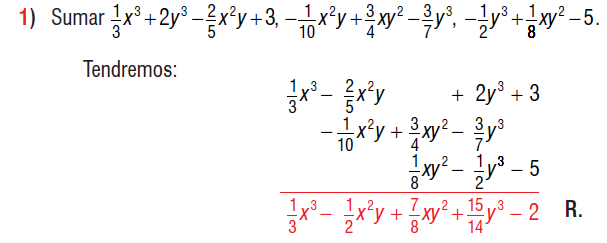
\includegraphics[scale=1.2]{Imagen1}
\caption{Fragmento tomado del Álgebra de Baldor}
\end{figure}
\begin{displaymath}
\renewcommand{\arraystretch }{2}
\begin{array}{ccccc>{\columncolor{gray}}p{1cm}}
\dfrac{1}{3}x^3&-\dfrac{2}{5}x^2y&&+2y^3&+3&\\
&\cellcolor{gray}\textcolor{white}{-\dfrac{1}{10}x^2y}&+\dfrac{3}{4}xy^2&-\dfrac{3}{7}y^3&&\\
&&\dfrac{1}{8}xy^2&-\dfrac{1}{2}y^3&-5&\\ \cline{1-5}
&&&&& \textcolor{white}{\textbf{R.}}
\end{array}
\end{displaymath}
% Please add the following required packages to your document preamble:
% \usepackage[table,xcdraw]{xcolor}
% Beamer presentation requires \usepackage{colortbl} instead of \usepackage[table,xcdraw]{xcolor}
\lipsum[1-10]
\section*{Vectores y Matrices}
\addcontentsline{toc}{section}{Vectore y Matrices} % Añade al índice
\markright{Vectores y Matrices}
\begin{figure}[H]
\centering 
\includegraphics[scale=0.5]{Simetria}
\caption{Esta imagen fue tomada de la página de internet \href{https://www.freepik.com/}{$\underline{Enlace}$}}
\end{figure}
\begin{center}
\fbox{
\begin{minipage}{0.7\textwidth}
Aunque no lo parezca, una imagen\index{imagen} no es más que una tabla de números para un computador.
\end{minipage}
}
\end{center}
\begin{Def}[Vector]
Se define un vector $x$ de $n$ elementos como una lista de $n$ números dispuestos de la siguiente forma:
\begin{displaymath}
x=
\begin{pmatrix}
x_1\\
x_2\\
\vdots\\
x_n
\end{pmatrix}
\end{displaymath}
Se denota que $x\in\mathbb{R}^n$.
\end{Def}
\begin{table}
\centering
\begin{tabular}{|c|c|c|}
\hline
1 & 2 & 3\\
\hline
\end{tabular}
\end{table}
Esta es la primera referencia\cite{ref1}
\cite{ref2}
\begin{thebibliography}{99}
    \bibitem[Referencia 1]{ref1} Autor A. Título del libro. Editorial, Año.
    \bibitem{ref2} Autor B. Título del artículo. Revista, Volumen (Número), Páginas, Año.
    \bibitem{ref3} Autor C. Título de la conferencia. Nombre de la conferencia, Lugar, Año.
    \bibitem{ref4} Autor A. Título del libro. Editorial, Año.
    \bibitem{ref5} Autor B. Título del artículo. Revista, Volumen (Número), Páginas, Año.
    \bibitem{ref6} Autor C. Título de la conferencia. Nombre de la conferencia, Lugar, Año.
    \bibitem{ref7} Autor XYZ. Título de la tesis. Universidad, Año.
        \bibitem{ref8} Autor C. Título de la conferencia. Nombre de la conferencia, Lugar, Año.
    \bibitem{ref8} Autor XYZ. Título de la tesis. Universidad, Año.
        \bibitem{ref9} Autor C. Título de la conferencia. Nombre de la conferencia, Lugar, Año.
    \bibitem{ref10} Autor XYZ. Título de la tesis. Universidad, Año.
    \bibitem{ref11} Autor A. Título del libro. Editorial, Año.
    \bibitem{ref12} Autor B. Título del artículo. Revista, Volumen (Número), Páginas, Año.
    \bibitem{ref13} Autor C. Título de la conferencia. Nombre de la conferencia, Lugar, Año.
    \bibitem{ref14} Autor A. Título del libro. Editorial, Año.
    \bibitem{ref15} Autor B. Título del artículo. Revista, Volumen (Número), Páginas, Año.
    \bibitem{ref16} Autor C. Título de la conferencia. Nombre de la conferencia, Lugar, Año.
    \bibitem{ref17} Autor XYZ. Título de la tesis. Universidad, Año.
        \bibitem{ref98} Autor C. Título de la conferencia. Nombre de la conferencia, Lugar, Año.
    \bibitem{ref19} Autor XYZ. Título de la tesis. Universidad, Año.
        \bibitem{ref18} Autor C. Título de la conferencia. Nombre de la conferencia, Lugar, Año.
    \bibitem{ref20} Autor XYZ. Título de la tesis. Universidad, Año.    
        \bibitem{ref21} Autor A. Título del libro. Editorial, Año.
    \bibitem{ref22} Autor B. Título del artículo. Revista, Volumen (Número), Páginas, Año.
    \bibitem{ref23} Autor C. Título de la conferencia. Nombre de la conferencia, Lugar, Año.
    \bibitem{ref24} Autor A. Título del libro. Editorial, Año.
    \bibitem{ref95} Autor B. Título del artículo. Revista, Volumen (Número), Páginas, Año.
    \bibitem{ref26} Autor C. Título de la conferencia. Nombre de la conferencia, Lugar, Año.
    \bibitem{ref27} Autor XYZ. Título de la tesis. Universidad, Año.
        \bibitem{ref98} Autor C. Título de la conferencia. Nombre de la conferencia, Lugar, Año.
    \bibitem{ref29} Autor XYZ. Título de la tesis. Universidad, Año.
        \bibitem{ref96} Autor C. Título de la conferencia. Nombre de la conferencia, Lugar, Año.
    \bibitem{ref30} Autor XYZ. Título de la tesis. Universidad, Año.
       \bibitem{ref31} Autor A. Título del libro. Editorial, Año.
    \bibitem{ref32} Autor B. Título del artículo. Revista, Volumen (Número), Páginas, Año.
    \bibitem{ref33} Autor C. Título de la conferencia. Nombre de la conferencia, Lugar, Año.
    \bibitem{ref34} Autor A. Título del libro. Editorial, Año.
    \bibitem{ref35} Autor B. Título del artículo. Revista, Volumen (Número), Páginas, Año.
    \bibitem{ref36} Autor C. Título de la conferencia. Nombre de la conferencia, Lugar, Año.
    \bibitem{ref37} Autor XYZ. Título de la tesis. Universidad, Año.
        \bibitem{ref58} Autor C. Título de la conferencia. Nombre de la conferencia, Lugar, Año.
    \bibitem{ref39} Autor XYZ. Título de la tesis. Universidad, Año.
        \bibitem{ref66} Autor C. Título de la conferencia. Nombre de la conferencia, Lugar, Año.
    \bibitem{ref40} Autor XYZ. Título de la tesis. Universidad, Año.
\end{thebibliography}
\printindex
\addcontentsline{toc}{chapter}{Índice Alfabético}
\end{document}
